\chapter{Potpourri}

Technique used to increase the model size, without significantly
increasing the computational cost of its execution.

We add many “experts” to the model e.g. different versions of one layer


Only one (or few) experts are used for any prediction.
Sparse Mixture of Experts (not using all experts!)

Originally proposed some time ago (Jacobs et al., 1991). Now used for LLMs, with some adaptations

\section{Expert layers in transformers}


\begin{flushleft}
  \begin{minipage}{0.65\linewidth}

    For transformer-based architectures, we often use different experts for the FF-NN layers.
    We need a way to know “who are the right
    experts”. Multiple experts can be selected (top-k), If k > 1, we must define how much we weight each expert's contribution

    We introduce a gating mechanism, a layer that decides, for each token, which experts should be used


  \end{minipage}%
  \hfill
  \begin{minipage}{0.3\linewidth}
    \centering
    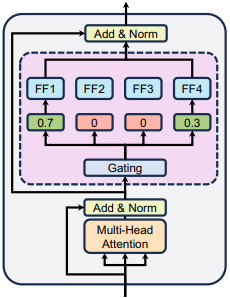
\includegraphics[width=1\linewidth]{content/Parts/images/2026-11-02-10-47-43.png}
  \end{minipage}
\end{flushleft}


\section{Gating mechanism}

\begin{flushleft}
  \begin{minipage}{0.65\linewidth}

    Each expert has a “gating vector”.

    Each token is scored against the gating
    vector (dot product)

    The top k experts are selected, and scaled
    (via sofmtax)

    The output is the weighted sum of the
    outputs of the selected experts


  \end{minipage}%
  \hfill
  \begin{minipage}{0.3\linewidth}
    \centering
    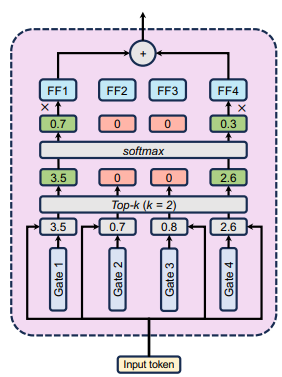
\includegraphics[width=1\linewidth]{content/Parts/images/2026-11-02-10-49-28.png}
  \end{minipage}
\end{flushleft}


\section{Mixtral}


\begin{flushleft}
  \begin{minipage}{0.65\linewidth}

    Sparse Mixture of Experts (SMoE)
    released by Mistral AI

    Based on Mistral 7B architecture

    8 experts in all FF-NN layers
    of transformers


    Top 2 experts selected

    Total parameters: 47B

    Active parameters at inference: 13B

  \end{minipage}%
  \hfill
  \begin{minipage}{0.3\linewidth}
    \centering
    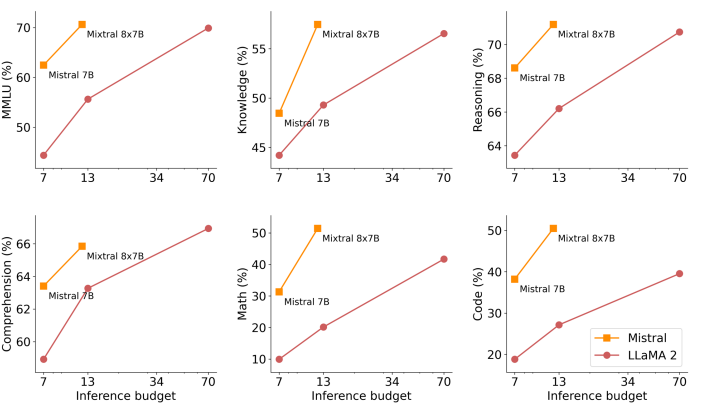
\includegraphics[width=1\linewidth]{content/Parts/images/2026-11-02-10-55-02.png}
  \end{minipage}
\end{flushleft}

\section{Vision-Language Models (VLM)}

VLM are multimodal models that can use both images and text as
inputs and/or outputs.


Used for a wide variety of tasks. Image captioning, Visual Question Answering, image-text matching.

Key components

\begin{itemize}
  \item Vision encoder (converts images to vectors)
  \item Language encoder (converts text to vectors)
  \item Multimodal fusion (combines vision and language vectors)
\end{itemize}

\section{CLIP}


\begin{flushleft}
  \begin{minipage}{0.65\linewidth}


    Contrastive Language Image Pretraining (CLIP) is one of
    the earlier vision-language models based on transformers ( OpenAI, 2021).

    Text and images are aligned in the same vector space. So that the vector of the image of a dog and the vector for the sentence “a picture of a dog” are close in the shared space.

    Vision modality (images) encoded with a vision encoder. ResNet, or Vision Transformer (ViT)

    Text modality encoded with a decoder-only model (simil
    GPT-2). Using vector associated to [EOS] token as representative of the text

    Similarity between text and images performed with
    cosine similarities



  \end{minipage}%
  \hfill
  \begin{minipage}{0.3\linewidth}
    \centering
    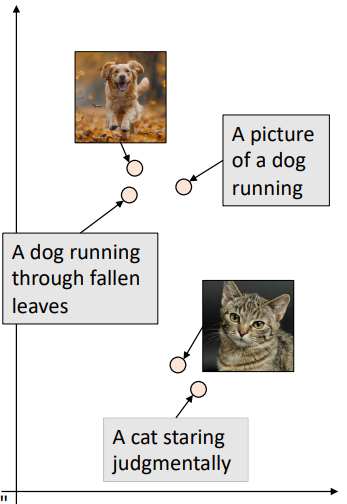
\includegraphics[width=1\linewidth]{content/Parts/images/2026-11-02-11-07-53.png}
  \end{minipage}
\end{flushleft}


\section{Contrastive learning alignment}

last 3 slide



